\documentclass[draft]{article}\usepackage[]{graphicx}\usepackage[]{color}
%% maxwidth is the original width if it is less than linewidth
%% otherwise use linewidth (to make sure the graphics do not exceed the margin)
\makeatletter
\def\maxwidth{ %
  \ifdim\Gin@nat@width>\linewidth
    \linewidth
  \else
    \Gin@nat@width
  \fi
}
\makeatother

\definecolor{fgcolor}{rgb}{0.345, 0.345, 0.345}
\newcommand{\hlnum}[1]{\textcolor[rgb]{0.686,0.059,0.569}{#1}}%
\newcommand{\hlstr}[1]{\textcolor[rgb]{0.192,0.494,0.8}{#1}}%
\newcommand{\hlcom}[1]{\textcolor[rgb]{0.678,0.584,0.686}{\textit{#1}}}%
\newcommand{\hlopt}[1]{\textcolor[rgb]{0,0,0}{#1}}%
\newcommand{\hlstd}[1]{\textcolor[rgb]{0.345,0.345,0.345}{#1}}%
\newcommand{\hlkwa}[1]{\textcolor[rgb]{0.161,0.373,0.58}{\textbf{#1}}}%
\newcommand{\hlkwb}[1]{\textcolor[rgb]{0.69,0.353,0.396}{#1}}%
\newcommand{\hlkwc}[1]{\textcolor[rgb]{0.333,0.667,0.333}{#1}}%
\newcommand{\hlkwd}[1]{\textcolor[rgb]{0.737,0.353,0.396}{\textbf{#1}}}%

\usepackage{framed}
\makeatletter
\newenvironment{kframe}{%
 \def\at@end@of@kframe{}%
 \ifinner\ifhmode%
  \def\at@end@of@kframe{\end{minipage}}%
  \begin{minipage}{\columnwidth}%
 \fi\fi%
 \def\FrameCommand##1{\hskip\@totalleftmargin \hskip-\fboxsep
 \colorbox{shadecolor}{##1}\hskip-\fboxsep
     % There is no \\@totalrightmargin, so:
     \hskip-\linewidth \hskip-\@totalleftmargin \hskip\columnwidth}%
 \MakeFramed {\advance\hsize-\width
   \@totalleftmargin\z@ \linewidth\hsize
   \@setminipage}}%
 {\par\unskip\endMakeFramed%
 \at@end@of@kframe}
\makeatother

\definecolor{shadecolor}{rgb}{.97, .97, .97}
\definecolor{messagecolor}{rgb}{0, 0, 0}
\definecolor{warningcolor}{rgb}{1, 0, 1}
\definecolor{errorcolor}{rgb}{1, 0, 0}
\newenvironment{knitrout}{}{} % an empty environment to be redefined in TeX

\usepackage{alltt}

\usepackage{graphicx}
\usepackage{wrapfig}

\graphicspath{ {images/} }

\title{Quick Tour of R and R Studio}
\date{February 12, 2106}
\author{Robert Olendorf}
\IfFileExists{upquote.sty}{\usepackage{upquote}}{}
\begin{document}
  \maketitle
  
  \pagenumbering{gobble}
  \newpage
  
  \section{R Studio}
  

  
  R Studio is an Integrated Development Environment (IDE) for the R Statistical Package. You can run R 
  fine from the command line and using text editors such as Notepad++ or Textmate, but it provides a 
  nice comprehensive view of your current project. It's also probably easier for beginners to learn on.
  
  \begin{figure}[t]
    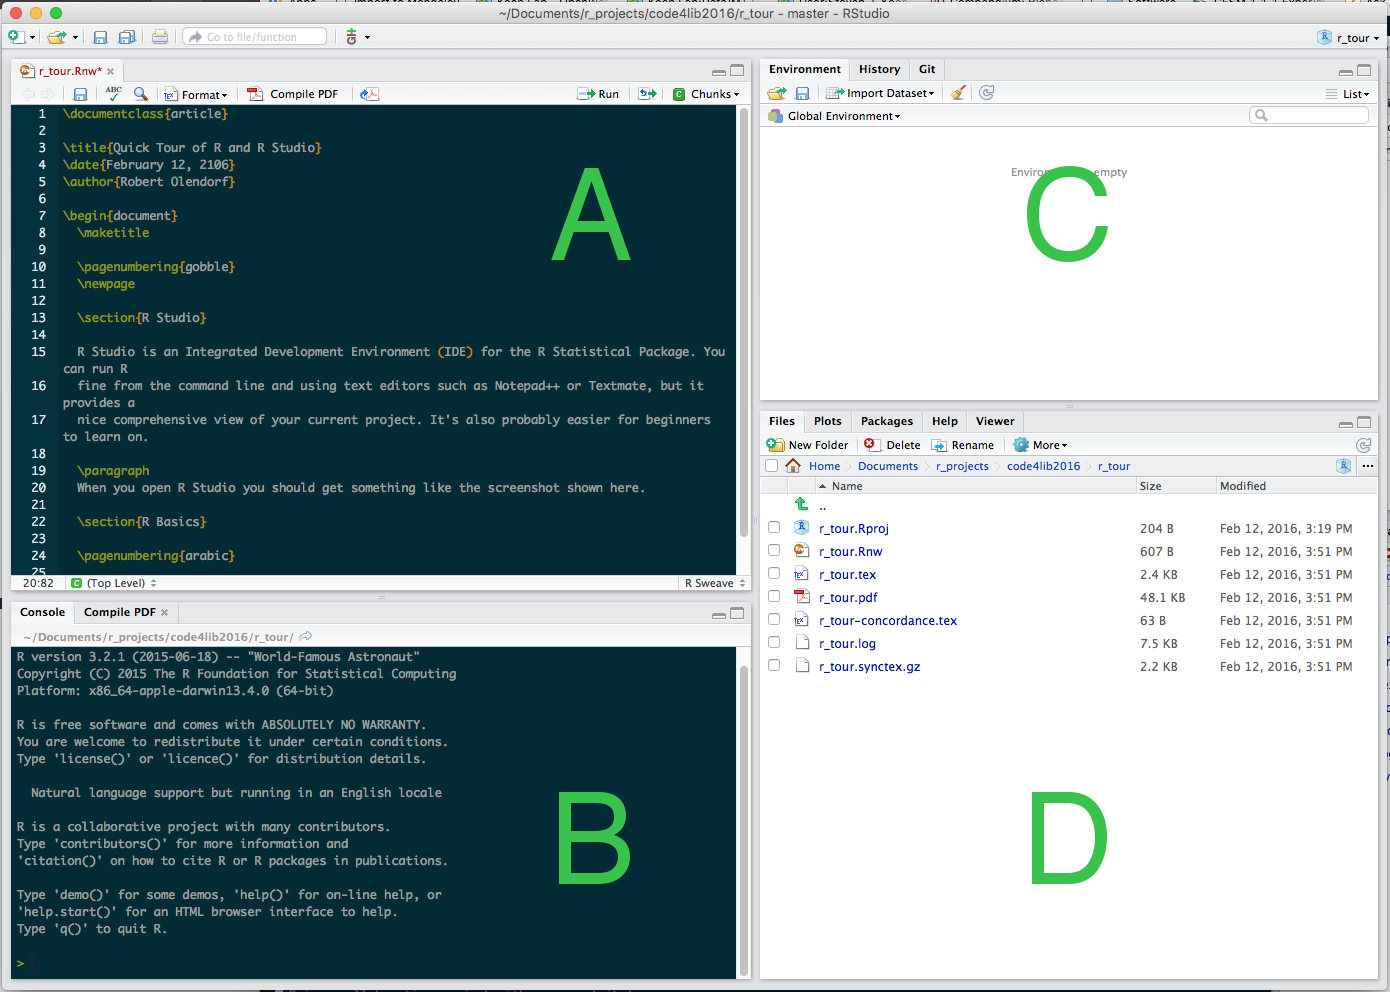
\includegraphics[scale=0.25]{rstudio_screenshot}
    \caption{Screen shot from the typical default layout.}
    \label{fig:screenshot}
    \centering
  \end{figure}
  
 When you open R Studio you should get something like the screenshot shown in figure \ref{fig:screenshot}. \textbf{Section A} is where your scripts and other documents are displayed. \textbf{Section B} is the \textbf{\textit{Console}}, where you do your interactive programming. \textbf{Section C} contains several tabs. It will usually contain at least your \textbf{\textit{Environment}}, a listing of all your objects (ie. variables, data) and a \textbf{\textit{History}} tab for your \textbf{\textit{Console}} input. \textbf{Section D} contains a number of tabs. Minimally it will contain a \textbf{\textit{Files}} tab, a \textbf{\textit{Plots}} tab, a \textbf{\textit{Packages}} tab, and a \textbf{\textit{Help}} tab. The \textbf{\textit{Files}} tab allows you to easily navigate the directory structure of your project. The \textbf{\textit{Plots}} tab displays previews of plots you generate. The \textbf{\textit{Packages}} tab lets you easily manage your R packages. The \textbf{\textit{Help}} tab displays the help.
 
 Our first task is to define a default working direcotry. This is where R will start when you are not working on a project. Opening and saving files will be relative to this directory. Choose \textbf{[Preferences]} from the \textbf{[RStudio]} menu.

  %Our first step will be to define a default working directory. This is where R will start, and save files if you are not working on a project. Choose \textbf{[Preferences]} the \textbf{[RStudio]} menu and choose the \textbf{[General]} tab. What I like to do is create a directory inside my Documents or what ever your call it directory called r_projects. 
  %After you have created the directory choose \textbf{[Browse\ldots]} and select it as your default working directory. Feel free to explore the other options as well. In particular I like to get my \textbf{Code}, \textbf{Appearance} set up to my liking. You might want to set up \textbf{Git/SVN}, but I prefer to use a separate terminal window to manage my versioning.
  
  %To get started lets open up a new project. Select \textbf{[File]} from the top menu and choose \textbf{[New Project\ldots]}. Choose the \textbf{New Directory} and \textbf{Empty Project} options. Then lets name the directory as \textit{hello_r} and \textbf{[Create Project]}.

  
  \section{R Basics}
  
  \pagenumbering{arabic}


\end{document}
